%
% Use the standard article template.
%
\documentclass{article}

% The geometry package allows for easy page formatting.
\usepackage{geometry}
\usepackage{float}
\geometry{letterpaper}


% Load up special logo commands.
\usepackage{doc}

% Package for formatting URLs.
\usepackage{url}

% Packages and definitions for graphics files.
\usepackage{graphicx}
\usepackage{epstopdf}
\DeclareGraphicsRule{.tif}{png}{.png}{`convert #1 `dirname #1`/`basename #1 .tif`.png}

%
% Set the title, author, and date.
%
\title{Headmaster Dream Design}
\author{Eric Dea}
\date{November 29, 2012}


%
% The document proper.
%
\begin{document}

% Add the title section.
\maketitle

% Add an abstract.
\abstract{
This paper explains my dream web interface for the headmaster web-app.  The headmaster web-app is an online database for a school that contains students info, events, grants, and other school related functions.  The paper will explain the top-level layout, a couple usage scenarios, reasons for the choices I make, and usability metrics.  These should effectively give the reader a good idea what my dream design is.  }

% Add various lists on new pages.
\pagebreak
\tableofcontents

\pagebreak
\listoffigures

\pagebreak

%
% Body text.
%
\section{Introduction}
\label{introduction}

In general, my dream design uses a mix of different interaction styles.  The choices for these styles has to do with the usability metrics in order to give the user the best experience using the web-app.  I do like the new interaction styles that involve the use of a computer's camera and speech.  Each interaction style has its own advantages and disadvantages.  Also, each user has a different mental model and experience with these interaction styles.  Thus, my dream design would like to incorporate the advantages of each interaction style to create a truly "perfect" interface.

\section{Top Level Design and Layout}

The design for my headmaster web-app is comprised of a login page, students page, grants page, events page, and a users page.

\subsection{Login Page}

For a new user or default settings, there is a standard form login design.  There are two fields, one for username and the other for password.  Inside the web-app, under the user settings, the user can edit their login preferences.  The preference options include a facial recognition login (built-in camera or attached camera through USB port), a speech recognition \cite{sphinx} login, the standard form filling login, or a combination of the three. Personally, I would use a combination of speech and facial recognition login. It provides a secure, and interesting way to login.  The form filling login is always visible to each user signing in, just in case the speech or facial recognition fail to work for some reason.

The background is default white, but can be changed in the user settings.  There will be a 'remember me' checkbox to save the username and background login image.  The facial recognition and speech login are available by default, but will not count as a valid login unless the user changes his/her preferences in the user preferences page.

\subsection{Welcome Page}

After the user logs in, the user will be brought to the welcome screen.  The page will have a 3D layout of a school (i.e. LMU), where the user can rotate, zoom, and click various sections of the school to bring up different pages.  The page would 'feel' like a virtual world where you see the school from a helicopter view. This layout uses direct manipulation to navigate around the virtual school.  

\begin{figure}[H]
\centering
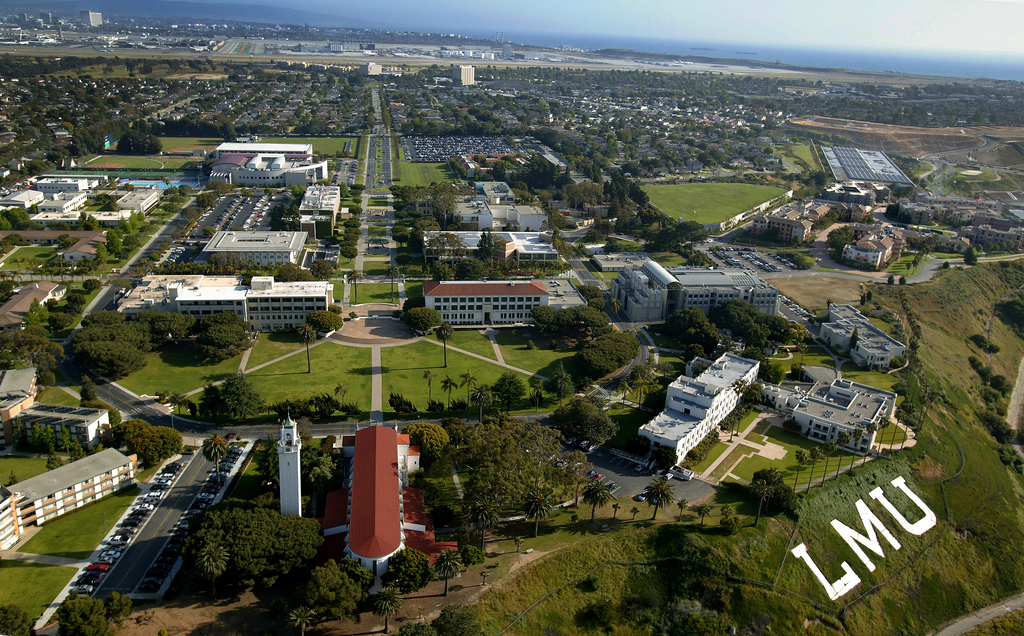
\includegraphics[width=4.5in]{LMU-Arial.jpg} 

\caption{LMU Arial view}
\label{LMU}
\end{figure}

The control are:

\begin{itemize}
\item Rotate: Click and drag the mouse.
\item Pan: Arrow Keys.
\item Zoom in/out: mouse scroll up/down.
\item Select buildings/links: Mouse click. 
\end{itemize}

The Student page link will be located in the dorm area as well as the admissions building.  The events page link is located in the Event Scheduling building.  The grants page link is located in the Financial aid office building.  The users page link is located in the registrar's office. 

In addition to just clicking the buildings to navigate to pages, the user can click a button in the top left to start the speech recognition.  The user can then say 'students' or 'users' to be directed to the page as well.  After saying the command, the speech software shows what it thinks the user says and then the user must confirm the request by saying 'yes' or 'correct.'  This reduces errors in saying the wrong command and being taken to the wrong page.

There is also a button in the top right that brings a drop down menu showing the previous links all at once.  This design incorporates direct manipulation with forms and menus.  The direct manipulation gives a cool and fun feel to the program while the menu drop-down gives a familiar more professional and familiar feel.

\subsection{Students}

The Student page is where the user can see the enrolled students.  Each student has a variety of information, such as major, address, email, etc.  So, my design for the Student page is a virtual world of students.  Essentially, each student is a created avatar model (similar to xbox 360 profiles and Miis from the Wii).  The user can add, delete or modify students.  In addition to all the information already included, there will be an option to include a picture of the student.  The picture is then associated to the student, and the avatar software (second life, weblin, etc.), along with facial recognition, takes the picture and puts it on the avatar's face.

\begin{figure}[H]
\centering
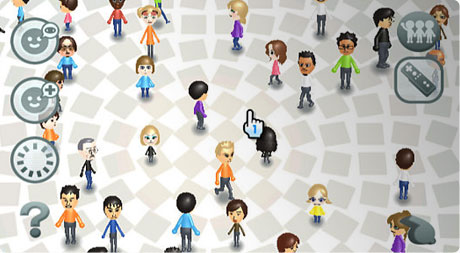
\includegraphics[width=4.5in]{Miis.jpg} 

\caption{Example of Student page}
\label{Mii}
\end{figure}

The layout will look like the Wii version of avatars, except not as cartoony.  I would like the avatars to have really good realism, similar to the current state of video games graphics (except for Wii, mainly PS3 and XBOX 360).  I like the idea of the avatars, or students, just hanging around waiting for the user to make an action.  The user would use different forms of direct manipulation to access the data of the students.  If the user finds the student on the screen, the user can click them and then the screen would go to the individual student page.  The information about each student is contained in forms, which can be edited by keyboard entry or speech (provided they click the speech button, which is contained to the right of each form).  The delete student button will be at the bottom of the screen, and when clicked, the user must confirm of the deletion in order to reduce errors.  There is a back button that brings the user to the lobby with all the other students. 

Creating a student is the same as editing a student, except the user will click a button to go to the creation screen.  In the lobby, the user can search for students in a variety of ways.  One way is manually panning and zooming the screen to find the student avatar 'walking' or 'hanging out' in the lobby.  The other way is using a search form.  The search form can be filled using the keyboard or speech.  The user can type or speak an student, major, or any information about the student to narrow down the number of avatars in the lobby.

\subsection{Events and Grants}

The Events and Grants pages are both similar in design.  The have a list of available events and grants, in text format.  For the events, however, there is a 3-dimensional calendar that shows each event in each day.  The calendar only shows the current month, and the user can switch between months by voice or mouse click.  The abilities of creation, editing, and deletion are basically the same as the student page. 

The Grants page is just a list of available grants.  The grants are categorized by qualification and amount.  Searching is available and can be used through speech command and/or a generic text form.

\subsection{Users}

The Users page lets users edit and change the preferences of each user.  There are two types of users, administrators and general users.  The page of the administrator is different than the general user.  The administrator page has a list of users to the left, each clickable by the mouse.  There is also a picture next to their username (if they provide a photo).  The admin can edit, delete, and add users at any time from the buttons on the top of the page.  This page does not have too much creativity, for admin is usually an experienced user and needs more functionality and efficiency than the general user.  

The general user page shows the current user's information in a 'security spider web' layout.  The web looks like a spider web in that the username is in the middle with all the information and preferences circling the middle.  They are attached to the middle by lines, or webs.  The color is a darkish blue with the webs being a lighter blue.  The layout is supposed to feel like a secure and safe program.  The ability to turn on speech and facial recognition is available on this page.  In order to use them, the webpage asks for specific information, like certain words for the voice recognition and a face picture for the facial recognition. 

\section{Usage Scenarios}

Two usage scenarios are for two different types of users: the administrator and the general user.

\subsection{Administrator}

The administrator would use this web-app to check the overall quality of his system.  Whether it be looking up students or editing users.  From the login screen, the experience is the same for everyone.  After logged in, the administrator can view students, check the available grants, see the events that students are having, and even check to see which students are registered for the web-app. 

\subsection{General User}

Most of the design choices are to affect the general user's experience.  From the login screen, the general user gets a sense of 'coolness' and instant familiarity due to the direct manipulation and voice recognition options.  The user is most likely to change his/her user preferences to voice and/or facial recognition, use the students page to find other students avatars, and to check out what events other students are having this month.  Since the experience is more social and fun, the experience should be the same.  Also while checking out the events, the navigation between the days and months of the calendar is seemingly fun.  The smoothness of the transitions between months and days is easily recognizable.  The welcome page is also both informative and very learnable.  Because of the navigation and links due to direct manipulation, the general user can navigate and find what he/she wants in minimal time.  Plus the 3D environment provides a pleasing view.

\section{Design Choices}

The design choices for my dream design interface are affected by many guidelines, principles, mental models, and concepts.

\subsection{Guidelines}

My user interface



 % Generate the bibliography.
\bibliography{cmsi370-dreamDesign}
\bibliographystyle{unsrt}

\end{document}
